\begin{frame}{}
\titlepage
\end{frame}

\begin{frame}{Table of Contents}
    \setbeamertemplate{section in toc}[sections numbered]
    \tableofcontents
\end{frame}

% ------
\section{Introduction}
% ------
\begin{frame}{Introduction}
    \begin{columns}
    \begin{column}{0.4\textwidth}
        \begin{itemize}[label=\textbullet]
            \item Item 1 in left column
        \end{itemize}
    \end{column}
    \begin{column}{0.7\textwidth}
        \begin{itemize}[label=\textbullet]
            \item Item 1 in right column
        \end{itemize}
    \end{column}
    \end{columns}
\end{frame}

\begin{frame}{Introduction}
    \textbf{Objectives:}
    \begin{itemize}[label=\textbullet]
        \item Objective 1
        \item Objective 2
    \end{itemize}
\end{frame}

% ------
\renewcommand{\sec}{New section}
\section{\sec}
% ------

\begin{frame}{\sec}
    \begin{itemize}[label=\textbullet]
        \item Time Independent Schrödinger Equation
        \begin{equation}
            \hat{H} \psi_i = E_i \psi_i
            .
        \end{equation}
        \item Hamiltonian of the symmetric double-well potential system
        \begin{equation}
            \hat{H} = - \frac{ \hbar^2 }{2 \mu} \frac{ \dd^2 }{ \dd{x^2} } + \frac{V_b}{x_e^4} x^4 - \frac{2V_b}{x_e^2} x^2 + V_b
            .
        \end{equation}
    \end{itemize}
\end{frame}

\begin{frame}{\sec}
    \begin{figure}[tb!]
        \centering
        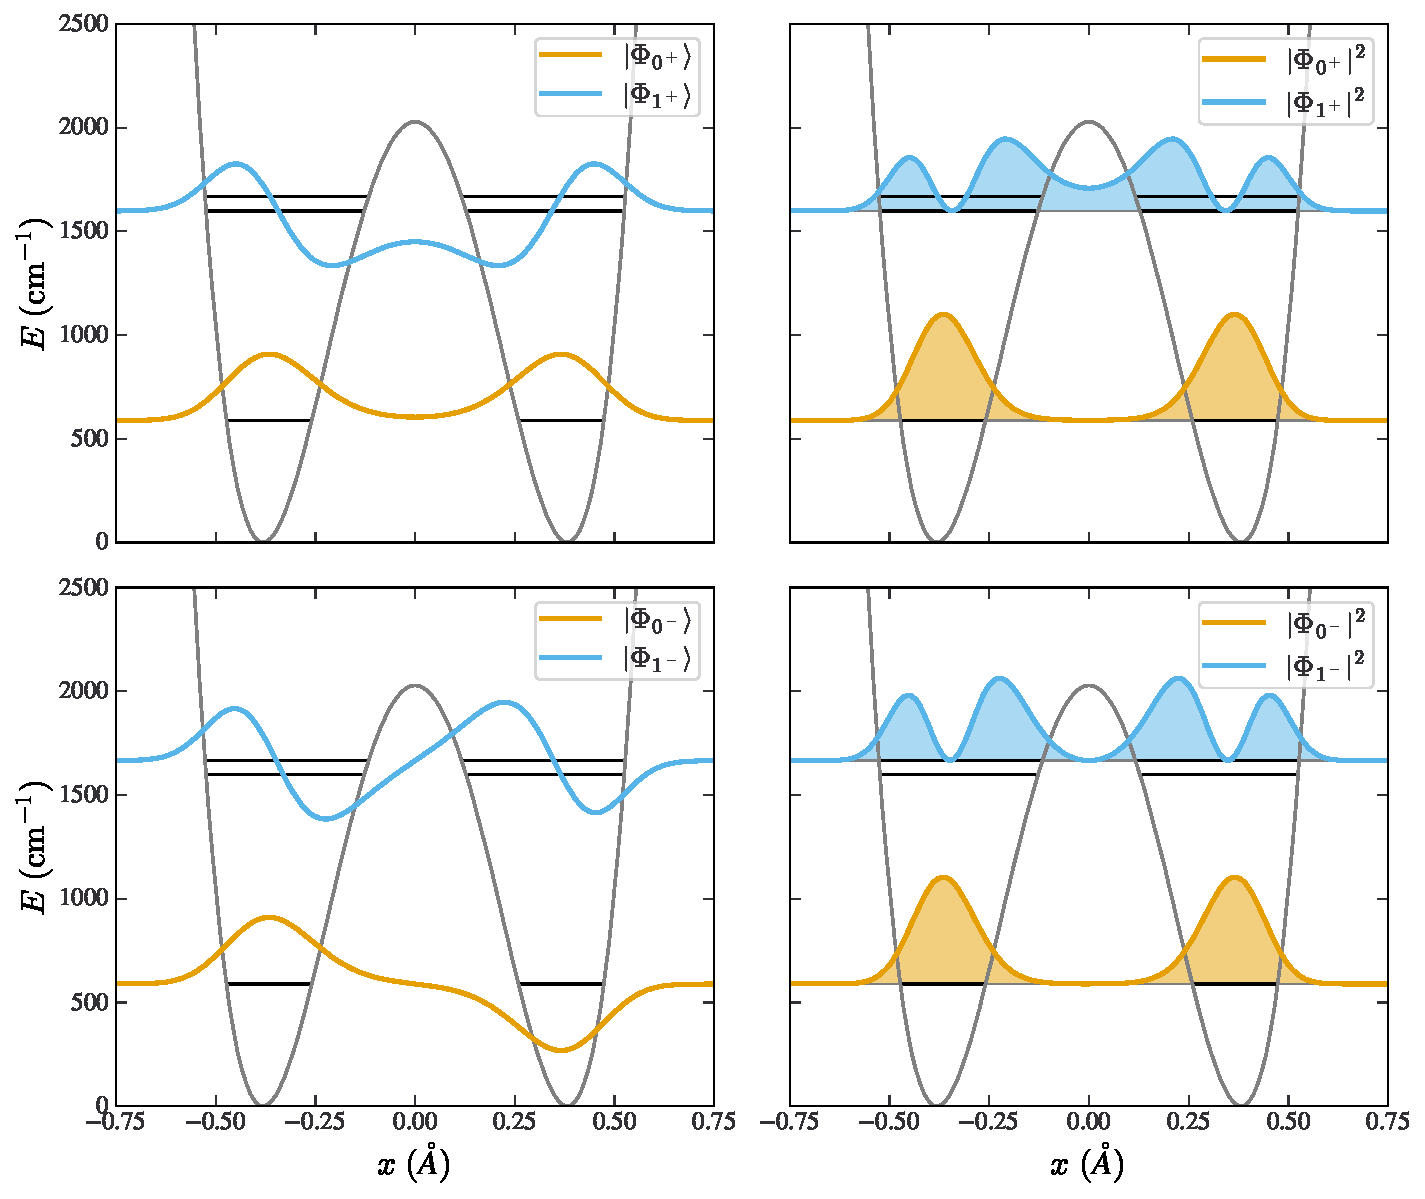
\includegraphics[width=1.0\textwidth]{fig1.pdf}
        % \subimport{figures/}{fig1.pdf.pgf}
        \caption{Eigenfunctions and probability densities.}
        \label{fig:fig1_pdf}
    \end{figure}
\end{frame}
